
\chapter*{The Hanging Chain and Quantum Bound States}
\addcontentsline{toc}{chapter}{The Hanging Chain and Quantum Bound States} 
\section*{Resonance for a hanging chain}
\addcontentsline{toc}{section}{Resonance for a hanging chain} 
	\marginpar{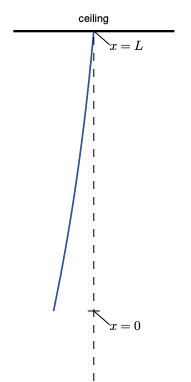
\includegraphics[width=\marginparwidth]{fig41}\captionof{figure}{The first normal mode for a hanging chain.}\label{fig:19}}

In the last lab, we studied waves on a string with constant tension and observed
sinusoidal normal modes of vibration. We\rq ll start off this lab by studying the
problem of standing waves on a hanging chain. It was the famous Swiss mathematician Johann Bernoulli who discovered in the 1700s that a draped hanging
chain has the shape of a \lq\lq catenary\rq\rq, or the hyperbolic cosine function. The problem of the normal mode frequencies of a vertical hanging chain was solved by
Johann\rq s son, Daniel Bernoulli, and is the first time that the function that later
became known as the $J_0$ Bessel function showed up in physics.
For a hanging chain, the tension varies with position—the tension at the top
is large (since it supports the weight of the whole chain) and the tension at the
bottom is essentially zero.1 We are going to find its normal modes of vibration of a
hanging chain using the method of Problem 3.3. The wave equation for transverse
waves on a chain with varying tension $T (x)$ and constant linear mass density $\mu$ is
given $by^2$

\begin{equation}\label{eq:41}
		\mu \frac{\partial^2 y}{\partial t^2} - \frac{\partial}{\partial x}(T(x)\frac{\partial y}{\partial x}) = 0
				\end{equation}
				
		We\rq ll use a coordinate system that defines $x = 0$ as the bottom of the chain and
$x = L$ as the ceiling.		

\paragraph*{P4.1}
Use the fact that a stationary hanging chain is in equilibrium to draw a
free-body diagram for a link at an arbitrary $x$. Use this diagram to show that
the tension in the chain as a function of $x$ is given by
	\begin{equation}\label{eq:42}
		T(x) = \mu g x
				\end{equation}		
				where $\mu$ is the linear mass density of the chain and $g = 9.8 m/s^2$
is the acceleration of gravity. Then show that Eq. \eqref{eq:41} reduces to	
	\begin{equation}\label{eq:43}
		 \frac{\partial^2 y}{\partial t^2} - g\frac{\partial}{\partial x}(x\frac{\partial y}{\partial x}) = 0
				\end{equation}	
				for a freely hanging chain.
			As in Lab 3, we now look for normal modes by separating the variables:
$y(x,t) = f(x)\cos(\omega t)$. We then substitute this form for $y(x,t)$ into \eqref{eq:43} and simplify to obtain	
		\begin{equation}\label{eq:44}
		 x \frac{d^2 f}{dx^2}+\frac{df}{dx} = - \frac{\omega^2}{g}f
				\end{equation}		
				which is in eigenvalue form with $ \lambda = −\omega^2/g$ . The boundary condition at the
ceiling is $f (L) = 0$ while the boundary condition at the bottom is obtained by
taking the limit of Eq. \eqref{eq:44} as $x \rightarrow 0$ to find
	\begin{equation}\label{eq:45}
		f^\prime(x) = - \frac{\omega^2}{g}f(0) = \lambda f(0)
				\end{equation}		
			\marginpar{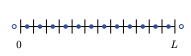
\includegraphics[width=\marginparwidth]{fig42}\captionof{figure}{A cell-centered grid with ghost points. (The open circles are the ghost points.)}\label{fig:20}}		
				In the past couple labs we dealt with derivative boundary conditions by fitting
a parabola to the last three points on the grid and then taking the derivative of
the parabola (e.g. Problems 2.4(b) and 3.4). This time we\rq ll handle the derivative
boundary condition by using a cell-centered grid with ghost points, as discussed
in Lab 1. Recall that a cell-center grid divides the spatial region from 0 to L into
N cells with a grid point at the center of each cell. We then add two more grid
points outside of $[0,L]$, one at $x_0  = −h/2$ and the other at $x_{N+1} = L + h/2$. The
ghost points are used to apply the boundary conditions. By defining N as the
number of interior grid points (or cells), we have $N +2$ total grid points, which
may seem weird to you. We prefer it, however, because it reminds us that we are
using a cell-centered grid with N physical grid points and two ghost points. \\
With this grid there isn\rq t a grid point at each endpoint, but rather we have two
grid points that straddle each endpoint. If the boundary condition specifies a
value, like $f (L) = 0 $ in the problem at hand, we use a simple average like this:
	\marginpar{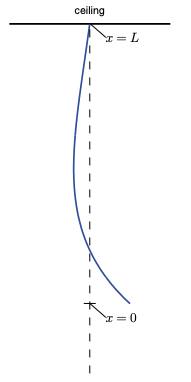
\includegraphics[width=\marginparwidth]{fig43}\captionof{figure}{The shape of the second mode of a hanging chain}\label{fig:21}}
\begin{equation}\label{eq:46}
		\frac{f_{N+1} + f_N}{2}=0
				\end{equation}	

For $f^\prime (L) = 0$, a centered derivative around $x = L$ yields
\begin{equation}\label{eq:47}
		\frac{f_{N+1} + f_N}{h}=0
				\end{equation}	
				\paragraph*{P4.2}
				\begin{enumerate}[label=(\alph*)]
			\item	On paper, write out the discretized version of Eq. \eqref{eq:44} and put it in
the form of a generalized eigenvalue problem
\begin{equation}\label{eq:48}
		Af = \lambda B f
				\end{equation}
					Remember that for the interior points, the matrix B is just the identity
matrix with 1 on the main diagonal and zeros everywhere else. Decide on the values needed in the bottom rows of A and B to give the
boundary condition in Eq. \eqref{eq:46} at $x = L$ (the ceiling) no matter what
$\lambda$ turns out to be.
	\marginpar{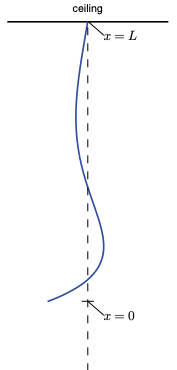
\includegraphics[width=\marginparwidth]{fig44}\captionof{figure}{The shape of the third mode of a hanging chain}\label{fig:22}}
\item Now let\rq s decide how to handle the derivative boundary condition at
$x = 0$ (the bottom of the chain), given by Eq. \eqref{eq:45}. Since this condition
is already in eigenvalue form we don\rq t load the top row of B with zeros.
Instead we load A with the left operator $f^\prime (0)$ according to Eq. \eqref{eq:47}
and B with the right operator $f(0)$  according to Eq. \eqref{eq:46}. Leave the
eigenvalue $ \lambda = − \omega ^ 2
/g$ out of the top row of B since the matrix equation
$Af = \lambda Bf$ already has the λ multiplying B. Write down the values
needed in the top rows of A and B, perform the matrix multiplication
for this row, and verify that your choices correctly produce Eq. \eqref{eq:45}.
\item Write a program to load the matrices A and B with $L = 2 m$ (or the measured length if different). Then solve for the normal modes of vibration
of a hanging chain. As in Lab 3, some of the eigenvectors are not physical because they don\rq t satisfy the boundary conditions; ignore them.
Compare your numerical resonance frequencies to measurements
made on the chain hanging from the ceiling in the classroom
\item The analytic solution to Eq. \eqref{eq:44} without any boundary conditions is
\begin{equation*}
		f(x) = c_1J_0(2\omega \sqrt{x / g}) + c_2 Y_0(2\omega \sqrt{2\omega \sqrt{x / g}})
				\end{equation*}
				where $J_0$ and $Y_0$ are the Bessel functions of the first and second kind,
respectively. The boundary condition at $x = 0$ rules out $Y_0$, since it is
singular at $x = 0$. Apply the condition $f(L) = 0$ to find analytically the
mode frequencies $ \omega_i$
in terms of the values xi that satisfy $J_0(xi) = 0$.
Verify that these values agree with the ω values from part (c).
HINT: The $scipy.special$ library has a function $jn_zeros(n,i)$
that will return the first $i$ values of $x$ for which $J_n(x)$ is zero.
				\end{enumerate}
				

\section*{Quantum bound states}
\addcontentsline{toc}{section}{Quantum bound states} 
Now let\rq s jump forward several centuries in physics history and study bound
quantum states using the same techniques we used to study the modes of a
hanging chain. Schrödinger\rq s equation for a potential well $V(x)$ is

\begin{equation}\label{eq:49}	
i \bar{h} \frac{\partial \Psi}{\partial t} = - \frac{\bar{h}^{2}}{2 m} \frac{\partial^{2} \Psi}{\partial x^{2}}+V(x) \Psi
				\end{equation}
				
		If we assume a separable solution of the form $\Psi(x,t) = \Psi(x)e^{
−i Et/ħ}$
and plug this
into Eq. \eqref{eq:49}, we find the time-independent Schrödinger equation

\begin{equation}\label{eq:410}
-\frac{\bar{h}^{2}}{2 m} \frac{d^{2} \psi}{d x^{2}}+V(x) \psi=E \psi
\end{equation}
For a particle in a one-dimensional harmonic oscillator, with $V (x) = kx^2/2$, this
becomes
\begin{equation}\label{eq:411}
-\frac{\bar{h}^{2}}{2 m} \frac{d^{2} \psi}{d x^{2}}+\frac{1}{2} k x^{2} \psi=E \psi
\end{equation}
with boundary conditions $\psi = 0$ at ±∞. Note that k is not the wave number; it is
the spring constant, $F = −kx$, with units of Newtons/meter.
The numbers that go into Schrödinger’s equation are so small that it makes
it difficult to tell what size of grid to use. For instance, using lengths like 2, 5, or
10 meters would be completely ridiculous for the bound states of an atom where
the typical size is on the order of $10^{−10}$ m. Some physicists just set $ħ, m$, and $k$
to unity, but this is bad practice. If you do this, you won\rq t know what physical
parameters your numerical results describe. The correct procedure is to \lq\lq rescale \rq\rq
the problem. \\ 
The goal of rescaling is to replace physical variables like x with unitless variables like $\xi = x/a$, where a is a \lq\lq characteristic \rq\rq length written in terms of the other
variables in the problem. Since a is a length, $\xi$ is unitless, and since a is scaled
to the problem parameters, $\xi$ will typically have magnitudes around the size of 1.
Let\rq s practice this procedure for the problem at hand.
	\marginpar{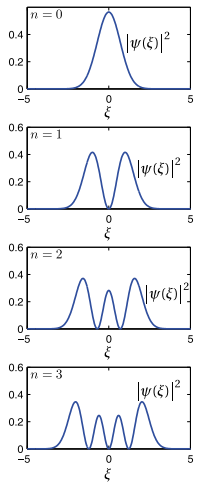
\includegraphics[width=\marginparwidth]{fig45}\captionof{figure}{The probability distributions for the ground state and the first three excited states of the harmonic oscillator.}\label{fig:23}}
\paragraph*{P4.3}  Substitute $x = \alpha \xi$ into Eq. \eqref{eq:411}, and then do some algebra to put the
equation in the form
\begin{equation}\label{eq:412}
-\frac{C}{2} \frac{d^{2} \psi}{d \xi^{2}}+\frac{1}{2} \xi^{2} \psi=\frac{E}{\bar{E}} \psi
\end{equation}
where the constants $C$ and $\bar{E}$ involve factors like $ħ, m, k$, and $a$.
Now make the differential operator on the left be as simple as possible by
choosing to make $C = 1$. This determines how the characteristic length a
depends on $ħ, m$, and $k$. Once you have determined a in this way, check to
see that it has units of length. You should find

\begin{equation}\label{eq:413}
a=\left(\frac{\bar{h}^{2}}{k m}\right)^{1 / 4}=\sqrt{\frac{\bar{h}}{m \omega}}, \quad \text { where } \quad \omega=\sqrt{\frac{k}{m}}
\end{equation}
Finally, rescale the energy by writing introducing a new variable $	\epsilon = E/\bar{E}$.
Show that $\bar{E}$ has units of energy, so that ϵ is unitless. You should find that
 \begin{equation}\label{eq:414}
\bar{E} = \bar{h}\sqrt{\frac{k}{m}}
\end{equation}
The final scaled version of Schrödinger\rq s equation then becomes
\begin{equation}\label{eq:415}
-\frac{1}{2} \frac{d^{2} \psi}{d \xi^{2}}+\frac{1}{2} \xi^{2} \psi=\epsilon \psi
\end{equation}
When you solve this equation and find results in terms of $\epsilon$ and $\xi$, you can
use the equations above to translate them into real-world values of E and x.\\
Now that Schrödinger\rq s equation is in dimensionless form, we are ready to
solve it with out standard technique.


\paragraph*{P4.4}
	\marginpar{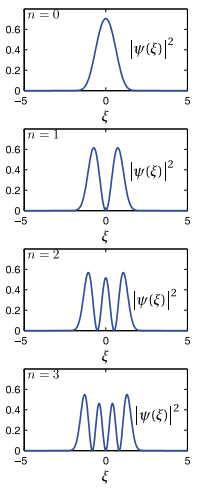
\includegraphics[width=\marginparwidth]{fig46}\captionof{figure}{The probability distributions for the ground state and the first three excited states for the potential in Problem 4.5}\label{fig:24}}
Discretize Eq. \eqref{eq:415} on paper. Then write a program to do this eigenvalue
problem, similar to the other programs we\rq ve written recently. The boundary conditions are that both the value and derivative of $\psi$ should go to zero
at $\xi$ = $\infty +$. Since you\rq ve scaled the problem, it makes sense to choose a
cell-edge grid that goes from $\xi =  - 5$ to $\xi  = 5$, or some other similar pair
of numbers. These numbers are supposed to approximate infinity in this
problem. Just set the value of $\psi$ to zero at the edge-points and make sure
(by looking at the eigenfunction solutions) that your grid is large enough
that the wave function has zero slope at the edges of the grid.


\begin{enumerate}[label=(\alph*)]
\item Plot the first several bound states. As a guide, Figure \ref{fig:23} displays the square
of the wave function for the first few excited states. (The amplitude has
been appropriately normalized so that $ \int |ψ(x)|^2 = 1$
\item  If you look in a quantum mechanics textbook you will find that the bound
state energies for the simple harmonic oscillator are given by the formula
\begin{equation}\label{eq:416}
E_n = (n + \frac{1}{2}) \bar{h}\sqrt{\frac{k}{m}} =(b+\frac{1}{2})\bar{E}
\end{equation}
so that the dimensionless energy eigenvalues $\epsilon_n$ are given by
\begin{equation}\label{eq:417}
\epsilon_n = n + \frac{1}{2}
\end{equation}
Verify that this formula for the bound state energies is correct for $n =
0,1,2,3,4$
\paragraph*{P4.5}
Now redo this entire problem, but with the harmonic oscillator potential
replaced by
\begin{equation}\label{eq:418}
V(x)=\mu x^4
\end{equation}
so that we have

\begin{equation}\label{eq:419}
-\frac{\bar{h}^{2}}{2 m} \frac{d^{2} \psi}{d x^{2}}+\mu x^{4} \psi=E \psi
\end{equation}
With this new potential you will need to find new formulas for the characteristic length and energy so that you can use dimensionless scaled variables as
you did with the harmonic oscillator. Choose a so that your scaled equation
is
\begin{equation}\label{eq:420}
- \frac{1}{2} \frac{d^{2} \psi}{d \xi^{2}} + \xi^{4} \psi = \epsilon \psi
\end{equation}

with $E = \epsilon \bar{3}$ . Use algebra by hand to show that

\begin{equation}\label{eq:421}
a=\left(\frac{\bar{h}^{2}}{m \mu}\right)^{1 / 6} \quad \bar{E}=\left(\frac{\bar{h}^{4} \mu}{m^{2}}\right)^{1 / 3}
\end{equation}
Find the first 5 bound state energies by finding the first 5 values of $ \epsilon_n $ in the
formula $E_n =  \epsilon_n \bar{E}$.

\end{enumerate}